\section{Inheritance}

\begin{frame}{New idea... new problem...}
    \begin{itemize}
        \pause
        \item We have now modeled a person with our \textit{Person} class
        \pause
        \item What if we want to model a student?
        \pause
        \item A student is also a person!
        \begin{itemize}
            \pause
            \item \textbf{Duplicate code}
        \end{itemize}
        \pause
        \item What is the best way to model this?
        \begin{itemize}
            \pause
            \item using \textbf{Inheritance!}
        \end{itemize}
    \end{itemize}
\end{frame}

\begin{frame}[plain]
So, what is inheritance?
\end{frame}

\begin{frame}{Inheritance}
    Lets look at the definition in the context of biology
    \pause
    \begin{block}{Inheritance (Biology)}
    Inheritance is the way that genetic information is passed from a parent to a child. Members of the same biological family tend to have similar characteristics
    \end{block}
\end{frame}

\begin{frame}{Inheritance}
    Lets translate this to OOP!
    \pause
    \begin{block}{Inheritance (OOP)}
    Inheritance is the concept in which a class can \textit{inherit} \textbf{data attributes} and \textbf{methods} from another class. Here, the class that inherits, is called the \textbf{derived class}. The class that the derived class inherits from, is called the \textbf{base class}.
    \end{block}
    \pause
    \begin{alertblock}{Alternative terminology}
        Inheriting is sometimes called \textbf{deriving}. So you can also say, the derived class \textbf{derives} data attributes and methods from it's base class.
    \end{alertblock}
\end{frame}

\begin{frame}{Inheritance}
    In the case of our example:
    \begin{block}{Inheritance (OOP)}
    Inheritance is the concept in which a class (\textbf{Student}) can \textit{inherit} data attributes (\textbf{first\_name, last\_name, age}) and methods (\textbf{speak()}) from another class (\textbf{Person}). The class that the derived class inherits from, is called the \textbf{base class}.
    \end{block}
    \begin{alertblock}{Alternative terminology}
        Inheriting is sometimes called \textbf{deriving}. So you can also say, the derived class \textbf{derives} data attributes and methods from it's base class.
    \end{alertblock}
\end{frame}

\begin{frame}{What can we do with inheritance?}
\begin{itemize}
    \item Create a \textbf{hierarchy} of classes (i.e. a class hierarchy :D) which describes their relationship (e.g. a Student is a Person, but not the other way around)
    \item Avoid writing duplicate code!
    \item \textbf{Encapsulation} (more on that later)
\end{itemize}    
\end{frame}

\begin{frame}[plain]
Let's look at the class hierarchy of our example!
\end{frame}

\begin{frame}{Hierarchies}
    \begin{figure}
        \centering
        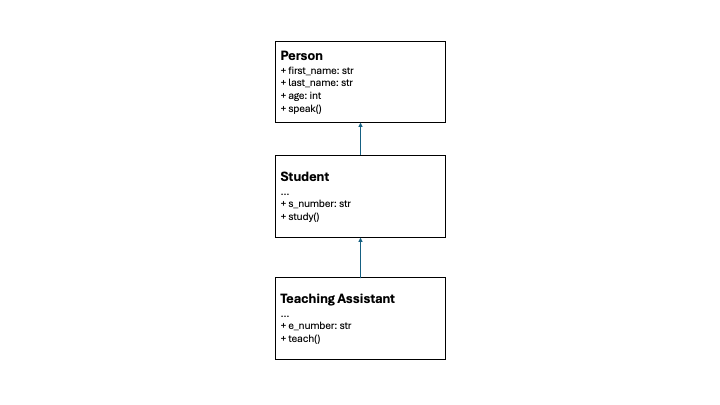
\includegraphics[scale=0.30]{images/hierarchy.png}
        \caption{our hierarchy}
        \label{fig:focuslogo}
    \end{figure}
    \pause
    \textbf{Note:} Inheriting classes (Student) can also be inherited from (TeachingAssistant)!
\end{frame}

\begin{frame}[plain]
Surprise quiz (no grade)
\end{frame}

\begin{frame}{Inheritance quiz}
What is the \textit{base class} of \textit{Student}?
\pause
\begin{itemize}
    \item \textbf{Answer:} Person
\end{itemize}
\pause
\person
Which class is \textit{Student} a \textit{derived class} of?
\pause
\begin{itemize}
    \item \textbf{Answer:} Person
\end{itemize}
\pause
What is a \textit{derived class} of \textit{Student}?
\pause
\begin{itemize}
    \item \textbf{Answer:} TeachingAssistant
\end{itemize}
\pause
Which data attributes does \textit{TeachingAssistant} inherit?
\pause
\begin{itemize}
    \item \textbf{Answer:} first\_name, last\_name, age, and s\_number
\end{itemize}
\pause
Which class is \textit{TeachingAssistant} a \textit{derived class} of?
\pause
\begin{itemize}
    \item \textbf{Answer:} Person and Student (sorry, it's both)
\end{itemize}
\end{frame}

\begin{frame}[plain]
How do we implement this in Python?
\end{frame}

\begin{frame}[fragile]{Remember our beautiful class}
\begin{minted}{python}
class Person():
    
    # The constructor
    def __init__(self, first_name, last_name, age):
        self.first_name = first_name  # Attribute
        self.last_name = last_name  # Attribute
        self.age = age  # Attribute

    # Method
    def speak(self):
        print(f"Hey, my name is {self.first_name}")
\end{minted}
\end{frame}

\begin{frame}[fragile]{Let's derive from it}
\begin{minted}[fontsize=\footnotesize]{python}
class Student(Person):

\end{minted}
\pause
\begin{minted}[fontsize=\footnotesize]{Python}
    # The constructor
    def __init__(self, first_name, last_name, age, s_number):
    
        # Calling the constructor of base class
        super().__init__(first_name, last_name, age)
        self.s_number = s_number

    # Method
    def study(self):
        print(f"Student {self.s_number} is studying!")
\end{minted}
\end{frame}

\begin{frame}{The super() function}
\begin{block}{super()}
The \textbf{super()} function refers to the base class of the class. We can use it to access/call methods of the base class.
\end{block}
If we call a method on the super() function, it is just like we would call it on \textbf{self}, but than as if it were an object of the base class!
\end{frame}

\begin{frame}[fragile]{Lets test it}
\pause
\begin{minted}[fontsize=\footnotesize]{python}
student = Student("Daan", "Wichmann", "secret", "secret")
\end{minted}
\pause
\begin{minted}[fontsize=\footnotesize]{python}
student.speak()
>>> Hey, my name is Daan
\end{minted}
\pause
\begin{minted}[fontsize=\footnotesize]{python}
student.study()
>>> Student secret is studying!
\end{minted}
\end{frame}

\begin{frame}{Hierarchies - Another example}
    \begin{figure}
        \centering
        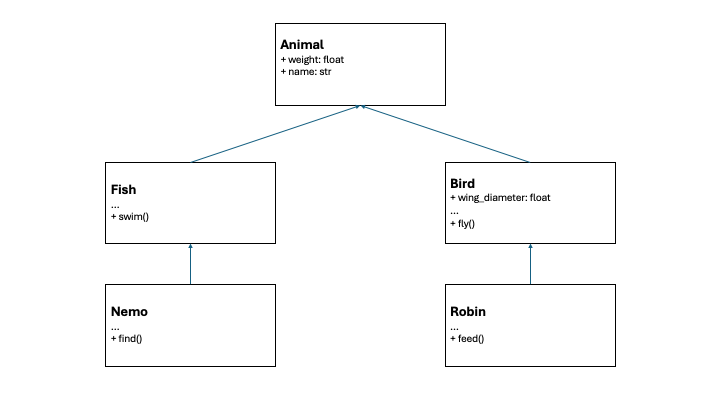
\includegraphics[scale=0.30]{images/hierarchy_another_example.png}
        \caption{Another example}
        \label{fig:focuslogo}
    \end{figure}
\end{frame}
